\documentclass[12pt,twoside]{article}
\usepackage[dvipsnames]{xcolor}
\usepackage{tikz,graphicx,amsmath,amsfonts,amscd,amssymb,bm,cite,epsfig,epsf,url}
\usepackage[hang,flushmargin]{footmisc}
\usepackage[colorlinks=true,urlcolor=blue,citecolor=blue]{hyperref}
\usepackage{amsthm,multirow,wasysym,appendix}
\usepackage{array,subcaption} 
% \usepackage[small,bf]{caption}
\usepackage{bbm}
\usepackage{pgfplots}
\usetikzlibrary{spy}
\usepgfplotslibrary{external}
\usepgfplotslibrary{fillbetween}
\usetikzlibrary{arrows,automata}
\usepackage{thmtools}
\usepackage{blkarray} 
\usepackage{textcomp}
\usepackage[left=0.8in,right=1.0in,top=1.0in,bottom=1.0in]{geometry}
\usepackage{pdfpages}

\title{Intro To Data Science: Data Analysis Project 1}
\author{Giulio Duregon / gjd9961}
\date{October 2021}

\newcommand{\R}{\mathbb{R}}

\begin{document}

\maketitle

\section{Introduction}
Dear Movie Company HQ Corporate,\\

We've received your instructions loud and clear, and will present our report that will answer all of your movie-related questions promptly. Being burgeoning data scientists myself, I consulted Pascal's lucky chart to guide our analysis. Pascal's chart is as follows:

\begin{figure}[h!]
    \centering
    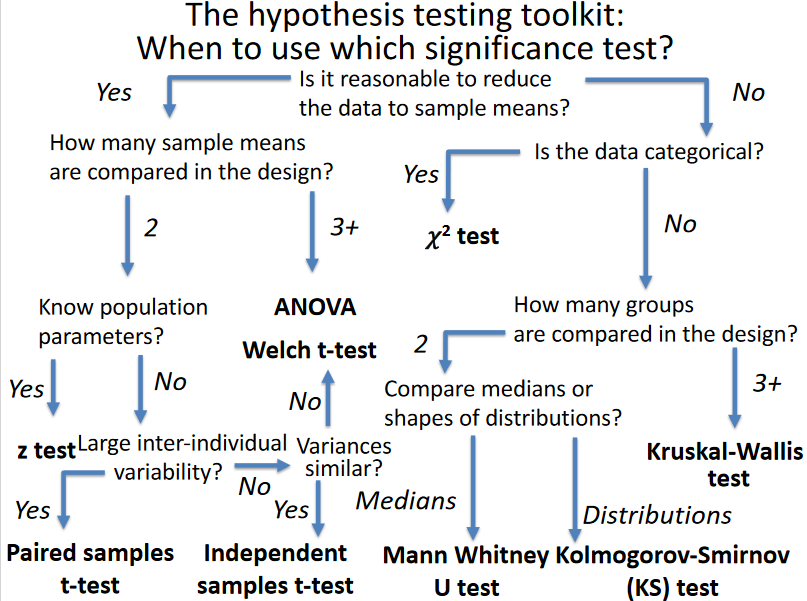
\includegraphics[scale=.6]{hypothesis testing.png}
    \caption{Pascal's Guide to Hypothesis Testing}
    \label{Pascal's Guide to Hypothesis Testing}
\end{figure}
This chart guided our decision making that you will see outline in the following report. Please don't fire me if my report ends up getting submitted for "Bad Data Science in the Wild".\\

\newpage 

\section{Report Findings: }
\begin{enumerate}
    \item   \textbf{Are movies that are more popular (operationalized as having more ratings) rated higher than movies that are less popular? }
    \subitem \textbf{Major Assumption: Movie Ratings Data should be considered categorical, as the mean is not meaningful}. Knowing this, I decided that it would be appropriate to consult Pascal's chart, which indicated the two tailed Chi Squared Test would be the perfect match to compare the two movie ratings. I conducted the test, and got a test statistic of 19600, and a p-value so small that it became rounded to 0. I decided to reject the null hypothesis, that the two groups of movies were rated the same, as our result was way below our alpha threshold. I concluded that indeed, more popular movies are rated higher.
    \item \textbf{Are movies that are newer rated differently than movies that are older?}
    \subitem Here I bifurcated our movie data yet again, this time on the release year. The median age was 1998, so I divided the 400 movies into two equal groups of 200 movies. Again, here the mean is not meaningful and there is plenty of data, so the Chi Squared Test was appropriate. Again, I found a statistically meaningful difference in the movies groups, with a test statistic of 76.5 and a p-value well below our alpha level. Again, I decided to reject the null hypothesis, that the old and new movies are rated the same. I concluded that old and new movies are rated differtly. 
    \item \textbf{Is enjoyment of ‘Shrek (2001)’ gendered, i.e. do male and female viewers rate it differently? }
    \subitem
    Again, I bifurcated our movie data, this time on gender, into two groups, male and female. The Chi-Squared Test was used again, and I found a significant difference of ratings for the movie 'Shrek (2001)' between male and female viewers. The test statistic was ~53, and the p-value again was well below our alpha threshold. I concluded to reject the null hypothesis, that female and male viewers did not rate Shrek differently. 
    \item \textbf{What proportion of movies are rated differently by male and female viewers?}
    \subitem 
    Again, movie data should be considered categorical, since the mean is not meaningful.(That's the last time I'm gonna say that). I wanted to conduct Chi-Squared tests on all the movies, between populations of males and females, but often times there wasn't enough data in each category to compare (I've heard that at least 5 observations per category are necessary to derive meaning from the Chi-Squared). Instead of the Chi-Squared Test, I performed the KS test, which I justified with Pascal's chart: the data was categorical but we couldn't do a Chi-Squared test, I was comparing two groups at a time, and I was not interested in the median rating (a Mann Whitney U Test), but rather the distribution. I found that that 6.25\% (25 out of 400) of movies had a statistically significant difference between the ratings of male and female viewers.  
    
    \newpage
    
    \item \textbf{ Do people who are only children enjoy ‘The Lion King (1994)’ more than people with siblings? }
    \subitem Here I again fell back to my trusty Chi-Squared test, for the aforementioned reasons. My null hypothesis was that there would be no difference in enjoyment of 'The Lion King (1994)' between only children and children with siblings. After performing the Chi-Squared test, I found a statistically significant difference between the ratings of each group, with a test statistic of 65 and an p-value way below our established alpha level. Again, I decided to reject the null hypothesis, and conclude that this difference was not due to chance alone. 
    \item \textbf{What proportion of movies exhibit an “only child effect”, i.e. are rated different by viewers with siblings vs. those without?}
    \subitem
    For this assignment I used the KS test yet again, as there was a significant lack of data so a Chi Squared Test was not viable. I found that .75\% (3 of 400) of movies had a significant difference in how they were rated between viewers with siblings and those without siblings.
    \item \textbf{Do people who like to watch movies socially enjoy ‘The Wolf of Wall Street (2013)’ more than those who prefer to watch them alone?}
    \subitem
    For this test, since we are interested in understanding if social viewers enjoyed the movie more, I decided to analyze the median of the ratings of each group. I used the Man Whitney U test, and found that there was a not a statistically significant difference in how social and non social viewers rated the movie (p-value .056). I did not reject the null hypotheses, and could not conclude that social viewers would rate 'The Wolf of Wall Street' more highly than non social watchers.
    \item \textbf{What proportion of movies exhibit such a “social watching” effect? }
    Here I utilized the KS test across all movies, and found that .5\% (2 out of 400) of movies exhibited a social watching effect.
    \item\textbf{ Is the ratings distribution of ‘Home Alone (1990)’ different than that of ‘Finding Nemo (2003)’? }
    \subitem
    Since we were interested in analyzing the distributions of the movies 'Home Alone (1990)' and 'Finding Nemo (2003)', I used the KS test. I found that there was a statistically significant difference, with an astronomically small p-value. I concluded that the distributions of ratings for the two movies were indeed different.
    \item \textbf{There are ratings on movies from several franchises ([‘Star Wars’, ‘Harry Potter’, ‘The Matrix’, ‘Indiana Jones’, ‘Jurassic Park’,  ‘Pirates of the Caribbean’, ‘Toy Story’, ‘Batman’]) in this dataset. How many of these are of inconsistent quality, as experienced by viewers?}
    \subitem
    For my methodology, I grouped each franchise into separate sections. I then iterated through each movie, comparing it to the others in the series, and measured if their distributions were statistically significantly different. I used the KS Test, and If any combination of movies in the franchise had a statistically significant difference, I would mark the series as inconsistent. I found that 2 of 8 franchises were consistent. The results are as follows:
    $$
        \begin{pmatrix}
            Movie & Consistent?\\
            \textit{Star Wars} & False \\
            \textit{Harry Potter} & True\\
            \textit{The Matrix} & False \\
            \textit{Indiana Jones} & False \\
            \textit{Jurassic Park} & False \\
            \textit{Pirates of the Caribbean} & True \\
            \textit{Toy Story} & False \\
            \textit{Batman} & False 
        \end{pmatrix}
    $$  
    \item (Extra Credit) 
    \subitem For the extra credit question I investigated whether there was a relationship between viewers who rated themselves highly (a rating of 3 or greater) in the "I have trouble following the story of a movie" section and how they rated movies. I looked to see if movies ratings were lower for that population and compared the ratings to their counterparts, (a rating of less than 3 for "I have trouble following the story of a movie" column). I found that only a single movie had a statistically significant difference, which was "The Sting (1973)". I used a KS test to determine if the distributions of each group were different, as there wasn't much data available for this field.  

\end{enumerate}

\end{document}
